\documentclass[11pt]{article}

\usepackage{report}

\usepackage[utf8]{inputenc} % allow utf-8 input
\usepackage[T1]{fontenc}    % use 8-bit T1 fonts
\usepackage[colorlinks=true, linkcolor=black, citecolor=blue, urlcolor=blue]{hyperref}       % hyperlinks
\usepackage{url}            % simple URL typesetting
\usepackage{booktabs}       % professional-quality tables
\usepackage{amsfonts}       % blackboard math symbols
\usepackage{nicefrac}       % compact symbols for 1/2, etc.
\usepackage{microtype}      % microtypography
\usepackage{lipsum}		% Can be removed after putting your text content
\usepackage{graphicx}
% \usepackage{natbib}
\usepackage{doi}
\usepackage{tabularx}
% \setcitestyle{aysep={,}}



\title{Toxic Comments Classification}

\author{Aarav Varshney and Argha Chakrabarty
\AND
\AND
	Ashoka University
}

% Uncomment to remove the date
\date{December 2021}

% Uncomment to override  the `A preprint' in the header
\renewcommand{\headeright}{Project Report}
\renewcommand{\undertitle}{Project Report}
\renewcommand{\shorttitle}{}

%%% Add PDF metadata to help others organize their library
%%% Once the PDF is generated, you can check the metadata with
%%% $ pdfinfo template.pdf
% \hypersetup{
% pdftitle={A template for the arxiv style},
% pdfsubject={q-bio.NC, q-bio.QM},
% pdfauthor={David S.~Hippocampus, Elias D.~Striatum},
% pdfkeywords={First keyword, Second keyword, More},
% }

\begin{document}
\maketitle

\newpage
\tableofcontents
\thispagestyle{empty}

\newpage
\thispagestyle{empty}

\setcounter{page}{1}
\section{Introduction}
The project presents an application of NLP to classify texts posted on online platforms as
comments as either toxic or non-toxic. While social media is a great medium for sharing opinions,
it is more and more being used to bully and harass people. This project aims to classify such comments
and hopefully make social media a bit more welcoming. We study the impact of tf-idf and SVMs, Decision Trees, Naive Bayes and CNNs.
We evaluated our approaches on comments from the \href{https://www.kaggle.com/c/jigsaw-toxic-comment-classification-challenge}{Kaggle Toxic Comments Classification Challenge}. Additionally
we host the classifier so that users can interact with it.


\section{Literature Survey}
\label{sec:headings}
This are several papers already published on the topic of Toxic Comments Classification. This was helpful for us to understand the topic and the way experts have approached it.
We have used the following papers for our analysis: 
\subsection*{Toxic Comment Classification by Zaher et al.}
The authors used Naive Bayes (as benchmark), RNN and LSTM to classify toxic comments. They trained the classifier on the same kaggle dataset. 
	\\
	\begin{tabular}{cc}
		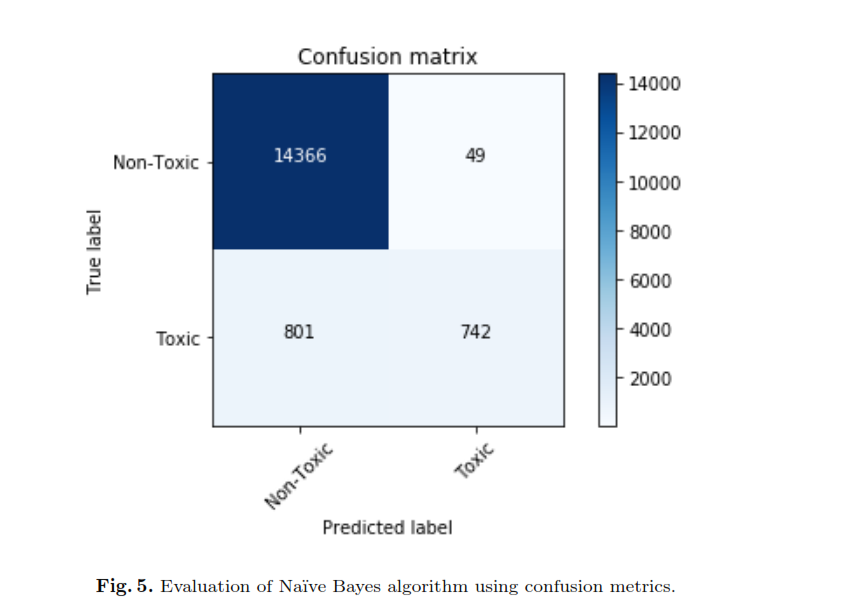
\includegraphics[width=65mm]{figs/zaher_bayes.png} & 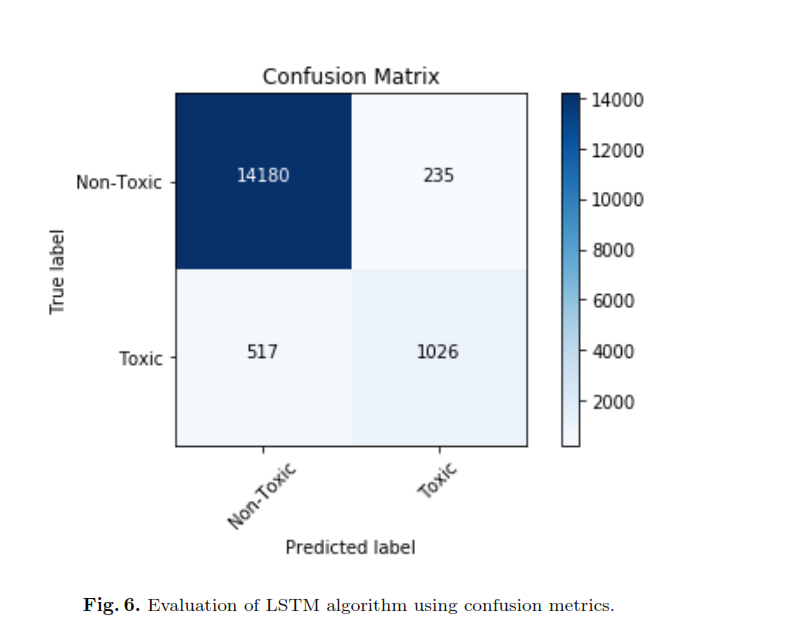
\includegraphics[width=65mm]{figs/zaher_lstm.png} 
	\end{tabular} \\
The results showed that LSTM has an almost 20\% increase in True Positive Rate (TRP) which means that among all the identified toxic comments
LSTM has 20\% more sensitivity in correct assignment of the comments. Furthemore there was an increase in Recall and F1 score when using LSTM.

\subsection*{A ML Approach to Comment Toxicity Classification by Chakrabarty}
The authors solved the problem of multi-label 
classification rather than binary and further classified toxic comments as hate, toxic, severelytoxic and so on. 
Two approaches were used for 3 labels each out of 6 labels. 
The authors used Bag of words using Word count vectorizer and then the tf-idf transformer which is finally used to train. Support Vector Machine (SVM) classifier with 100 as maximum iterations and C as 1.0. Whereas for the other three labels, decision tree classifier was used instead.

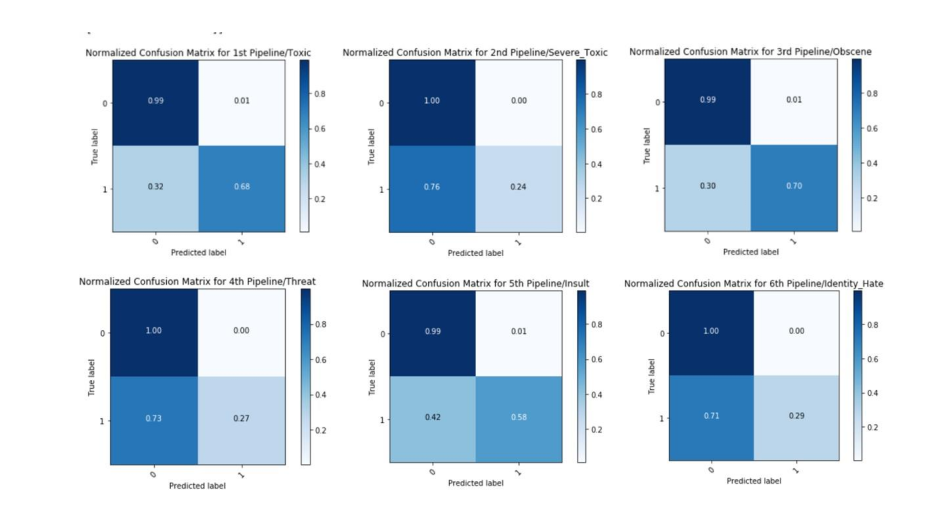
\includegraphics[scale=0.9]{figs/chakra_all.png}

The paper claims that this apporach performs better than
LSTM and Naive Bayes and the results validates this claim. 
We want to validate this claim on binary classification.
\section{Project Description and goals}
The project is to classify toxic comments on social media platforms. The goals are as follows:
\subsection*{Use Different Classification Techniques}
\begin{enumerate}
	\item \textbf{Naive Bayes}: Use the results as a benchmark to 
	compare other results with. This was chosen due to its reputation as a text classifier. This is a Generative Learning Algorithm that uses discrete values rather than continuous. Here we model p(x|y) that is the probability a particular word occurs given the comment is toxic or not. We make a strong assumption that xi's are conditionally independent given y. Finally after fitting the model, we calculate
	p(y = 1|x) which is just p(x|y = 1)p(y = 1)/ p(x)
	
	\item \textbf{Logistic Regression}: We wanted to try regression and for discrete values, we used logistic regression.
	\item \textbf{Decision Trees}: Here at each level we place the best feature at the node and then the split happens  depending on the features that produce the minimum classification error. And we chose the output based on the class of majority of data in the decision node.

	\item \textbf{Support Vector Machines}: Support vector machine models are unique in that they find the boundaries between classes by looking at the distances between the separating line and the nearest point for each class, and are resistant to outliers. 

\end{enumerate}
\subsection*{Deploy The Model}
Finally, we want to create REST API for the classifer that can be deployed on any platform. We used Flask for this.	

% <!-- DATASET SPECS -->

\section{Dataset Specification}
The dataset was acqured from Wikipedia comments which was then labelled by Jigsaw and then finally provided by Kaggle. The dataset had 1,59,571 comments, where each comment was labelled as toxic, severe toxic, obscene, threat, insult, identity hate or none. 
The data was labelled by the teams at Jigsaw (Alphabet) where each comment was labelled by at least 7 humans to reduce bias.
The length of each comment varied from 10 words to 1200 words. 
We ran an analysis to chose comments with
word count less than 600 as we saw that after this length, the number of toxic 
comments were too few. So, a total of 1,32,327 comments were chosen.
\begin{figure}[h]
\begin{center}
	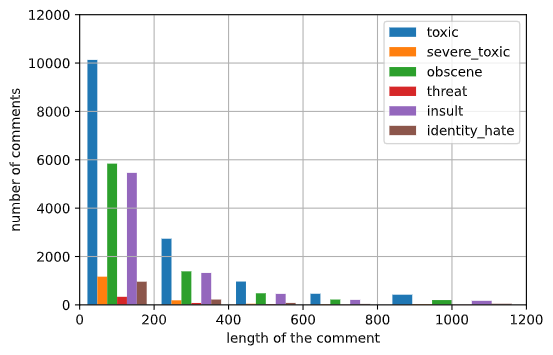
\includegraphics[scale=0.5]{figs/distribution.png}
	\caption{Length of comments}
	\label{fig:data_distribution}
\end{center}
\end{figure}

This is a multilabel classifier porblem which we converted to a binary classifier problem by relabelleing any comments identifying as any of the seven categories mentioned earlier. But the results for both have been published. \\
The dataset also went through stemming and lemmatization to remove any or all stopwords. Furthermore, we cleaned punctuations, numbers also ip-addresses as well attempted to remove usernames so that particular usernames do not make the model biased.\\
\begin{figure}[h]
	\begin{center}
		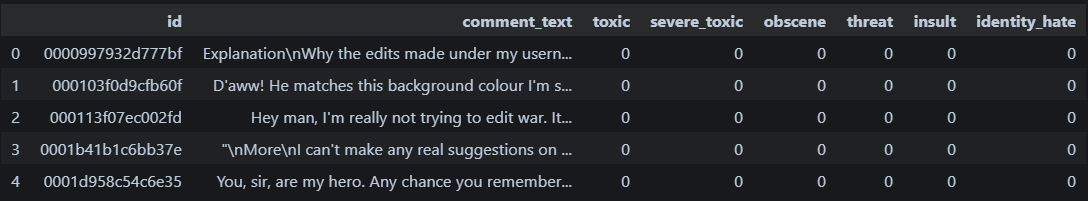
\includegraphics[scale=0.35]{figs/data_set.png}
		\caption{A snapshot of the dataset}
		\label{fig:dataset}
	\end{center}
\end{figure}

% <!-- Implementation -->


\section{Implementation details}
\subsection*{Data Preprocessing}
After the data is read, we select only comments with less than 600 words in it, 
and label each comment as toxic or not depending on the pre-existing labels.
nltk's wordnet module is used for stemming and lemmetizeing each comment 
after removing all the punctuations and numbers along with any other 
redundant utf-8 characters.
\subsection*{Vectorization} 
After all the comments are cleaned, we use TF-IDF to vectorize 
our comments so that we can use them for training our model. 
TfidfVectorizer is used as is from the scikit-learn module. TF-IDF stands for 
Term frequency-inverse document frequency, is a numerical statistic that is
intended to reflect how important a word is to a document in a collection.
A document in this case is the comment whether toxic or not. 
It does this by comparing the frequency of usage inside an individual comment
as opposed to the entire data set. 
The importance increases proportionally to the number of times a word appears in the 
individual coment which is called Term Frequency. 
But if multiple comments contain the same word repeatedly (example stopwords) 
then their importance decreases. 

\begin{quote}
TF(t) = Number of times term t appears in a document / Total number of terms in the document\\
IDF(t) = $log_e$(Total number of documents / Number of documents with term t in it). \\
Value = TF * IDF
\end{quote}
This vector becomes the feature vector for each comment. We further explored feature engineering where we can add features such as char length, word count, number of exclamations etc as features as well. We're leaving this out for now but we want to experiment more with feature engineering and see if it improves the results.

\subsection*{Training and Testing}
The test to train split ratio is 3:1. Then we trained our model on SVM, Logistic Regression, Naive Bayes and Decision Trees.
We trained the model on a laptop with i5-8520U and 16 gigs of RAM.
We also trained a multi-label model using Binary Relevence from scikit-multilearn module 
which is built on top of scikit-learn eco-system and provides multi label classification. \\
The dataset is heavily skewed to non-toxic comments (about 90\%) so a basic recall value will not be able to evaluate the model. We relied on Confusion Matrix and F1-Score which penalize the  models that just predict everything as either positive or negative with an imbalanced dataset.

\subsection*{Deployment}
After training, we decided to deploy our model for demo purposes. 
Since we used python for our project, we decided to go with a simple FastAPI server.
We created a pipeline with two stages, the first one vectorizing any
input text and at the stage the actual fitting or prediction occurs. 
To save the model we pickle the pipeline object using python's in-built 
pickle library and write the raw binary data onto a file. 
Afterwards, the file is un-pickled at the server-side and a single string 
array is given to it for prediction. 
The API takes a single string as it's payload and returns the predicted outcome 
as it's response. The user has to create a POST request with the comment as the 
payload and we return whether the comment is toxic or not in the response body.
Lastly we deployed the whole thing in a heroku server.
You can take a look at the API at this link 
:- \url{https://iml-tox-det.herokuapp.com/docs}
(please keep in mind that we are using a free server, it might take some time to start). 
We also went on and created a frontend website that uses the api: 
\url{https://adoring-bell-52f360.netlify.app}
\section{Observations}
\subsection*{Binary Classifcation}
\begin{tabularx}{0.8\textwidth} { 
	| >{\raggedright\arraybackslash}X 
	| >{\raggedright\arraybackslash}X 
	| >{\centering\arraybackslash}X 
	| >{\raggedleft\arraybackslash}X | }
	\hline
	Model & Recall & Precision & F1-Score \\
	\hline
	Naive Bayes & 0.985 & 0.272 & 0.426 \\
	\hline
	Logistic Regression  & 0.939  & 0.608 & 0.738  \\
	\hline
	Decision Tree & 0.751 & 0.71 & 0.73 \\
	\hline
	SVM & 0.926 & 0.653 & 0.766 \\
	\hline
\end{tabularx}

\section{Conclusions and future directions}
The results even though do not match that of the researchers, still give good results. SVM Model clearly performs better than the other models and our benchmark model. We wanted to explore some CNN models as well but since we wanted to deploy the model and use it for realtime testing, the model proved too slow for that. We also wanted to explore more feature engineering techniques and see if they would improve the results. Our future goal for the project is to test an LSTM model after fully understanding how it works and deploying it. We also want to incorportate some context detection techniques to improve the results where we analyze the context of the comment by analyzing the post, and the parent threads.  	

\bibliographystyle{unsrtnat}
\begin{thebibliography}{1}

	\bibitem{kour2014real}
	Zaheri, Sara; Leath, Jeff; and Stroud, David.
	\newblock Toxic Comment Classification,
	\newblock In {\em SMU Data Science 
	}, Review: Vol. 3 : No. 1 , Article 13

	\bibitem{kour2014fast}
	Navoneel Chakrabarty.
	\newblock A Machine Learning Approach to Comment
	Toxicity Classification 
	\newblock In {\em Jalpaiguri Government Engineering College, Jalpaiguri, West Bengal, India}

	\bibitem{hadash2018estimate}
	Kevin Khieu, Neha Narwal
	\newblock CS224N: Detecting and Classifying Toxic Comments
	\newblock In {\em Stanford University, Stanford, CA, USA}

	\bibitem{kour2018toxic}
	Prinslou Tare
	\newblock Toxic Comment Detection and Classification
	\newblock In {\em Department of Computer Science
	Stanford University}
\end{thebibliography}


\end{document}
